\chapter{Construção da Aplicação}\label{chp:des}

\section{Estudo de caso: principais assuntos e abordagens}

\subsection{Matrizes curriculares}



\textbf{Comparação e extração de assuntos em comum}

\textbf{Classificação por grau de relevância}

\textbf{Validação com professores do ensino fundamental I}

\begin{longtable}{|m{1.5cm}|m{3.5cm}|m{4.5cm}|m{5cm}|}
\hline
\textbf{Unidade} & \textbf{Tópico} & \textbf{Sobre esta unidade} & \textbf{Sugestões} \\
\hline
\endfirsthead

\hline
\textbf{Unidade} & \textbf{Tópico} & \textbf{Sobre esta unidade} & \textbf{Sugestões} \\
\hline
\endhead

\hline
\endfoot

\hline
\endlastfoot

I & Números: soma e subtração & Nessa unidade temática vamos estudar noções básicas de adição e subtração. & 
Antes iniciar as operações (adição, subtração, multiplicação, divisão) seria interessante trazer o sistema de numeração decimal: leitura, escrita, comparação e ordenação de números naturais de até cinco ordens. Usar o termo adição ao invés de soma. Depois de abordar essas duas operações separadamente vale relacionar as duas: adição e subtração. \\
\hline
II & Números: multiplicação e divisão & Nessa unidade temática vamos estudar noções de multiplicação e divisão. & 
Depois de abordar essas duas operações separadamente vale relacionar as duas: multiplicação e divisão. \\
\hline
III & Números: frações & Nessa unidade temática vamos estudar frações. & 
Trazer já aqui a representação decimal escrevendo valores do sistema monetário brasileiro. Isso ajudará na Unidade VIII de Educação Financeira. \\
\hline
IV & Álgebra & Nessa unidade temática vamos estudar padrões numéricos e determinar valores faltantes. & 
Usar o termo sequências numéricas ao invés de padrões numéricos. \\
\hline
V & Geometria & Nessa unidade temática vamos estudar paralelismo, área de superfícies, ângulos e algumas formas geométricas básicas. & 
Antes de paralelismo ajudaria iniciar reforçando conceitos como localização e movimentação: pontos de referência, direção e sentido. Depois das formas geométricas poderiam finalizar acrescentando os sólidos geométricos básicos conectando com suas planificações. \\
\hline
VI & Grandezas e medidas & Nessa unidade temática vamos estudar as principais unidades de medida. & 
Se possível trazer as 5 unidades de medida: comprimento, massa, capacidade, tempo e temperatura. \\
\hline
VII & Probabilidade e estatística & Nessa unidade temática vamos estudar gráficos e eventos aleatórios. & 
Antes de iniciar probabilidade trazer problemas de contagem simples que possam resolver por agrupamentos e escrita multiplicativa. \\
\hline
VIII & Educação financeira & Nessa unidade temática vamos estudar um pouco sobre educação financeira. & 
Trazer problemas utilizando o sistema monetário brasileiro. \\
\hline
IX (Bônus) & Algarismos romanos & Nessa unidade temática vamos aprender a ler algarismos romanos. & 
Achei ótimo esse bônus se possível acrescentar antes o sistema de numeração egípcio depois segue com o sistema de numeração romano. \\

\caption{Feedbacks e observações sobre o conteúdo e sua abordagem}




\end{longtable}

\textbf{Matriz de assuntos que irão ser abordados na aplicação após o estudo de casos}


\section{Comparativo de aplicações de ensino}

\textbf{Aplicação Duolingo}

Duolingo é uma plataforma de aprendizado de idiomas amplamente popular, acessível via website e aplicativos móveis. Fundada com o objetivo de tornar o aprendizado de idiomas acessível e divertido, a plataforma oferece uma maneira inovadora e gamificada de aprender novas línguas. 

\begin{enumerate}
    \item \textbf{Como Funciona}
    
    A metodologia do Duolingo baseia-se em atividades interativas e lições curtas que incentivam a prática diária. As lições são estruturadas em níveis e unidades, cobrindo aspectos como vocabulário, gramática, leitura, escrita e pronúncia. A gamificação é um componente crucial, com elementos como pontos, conquistas e um sistema de vidas que motiva os usuários a continuar aprendendo.

    \item \textbf{Tecnologias Inovadoras}

    O Duolingo se destaca por sua aplicação inovadora de tecnologias para aprimorar a experiência de aprendizado de idiomas:

    \begin{itemize}
        \item \textbf{Aprendizado de Máquina e Inteligência Artificial (IA):}
        \begin{itemize}
            \item \textbf{Algoritmos Adaptativos:} Personalizam o conteúdo e as atividades de acordo com o ritmo e estilo de aprendizado de cada usuário, otimizando a eficácia do ensino.
            \item \textbf{Avaliação Automática:} Oferece feedback instantâneo sobre a pronúncia e escrita, auxiliando na correção de erros e no aprimoramento contínuo.
            \item \textbf{Chatbots e Assistentes Virtuais:} Permitem a prática da conversação de forma interativa e personalizada, simulando situações reais de comunicação.
        \end{itemize}
        
        \item \textbf{Processamento de Linguagem Natural (PLN):}
        \begin{itemize}
            \item \textbf{Compreensão e Geração de Texto:} Possibilita a criação de exercícios e atividades que simulam a comunicação natural, como diálogos e textos escritos.
            \item \textbf{Análise Semântica:} Garante a precisão e relevância das traduções e do conteúdo apresentado aos usuários.
            \item \textbf{Reconhecimento de Fala:} Permite a avaliação da pronúncia e entonação do usuário, aprimorando suas habilidades orais.
        \end{itemize}

        \item \textbf{Gamificação:}
        \begin{itemize}
            \item \textbf{Sistemas de Pontos e Recompensas:} Motivam os usuários a continuar aprendendo e progredindo na plataforma.
            \item \textbf{Níveis e Desafios:} Criam um senso de conquista e engajamento, mantendo o interesse dos usuários.
            \item \textbf{Tabelas de Classificação e Competição Amistosa:} Estimulam a interação entre os usuários e promovem a colaboração.
        \end{itemize}
    \end{itemize}

    \item \textbf{UX/UI: Uma Experiência de Aprendizagem Intuitiva e Agradável}
    
    O Duolingo se preocupa em oferecer uma interface amigável e intuitiva que facilite o aprendizado:

    \begin{itemize}
        \item \textbf{Design Simples e Minimalista:} Prioriza a clareza e a organização da informação, evitando distrações e facilitando a navegação.
        \item \textbf{Recursos Visuais Atraentes:} Utiliza cores vibrantes, ilustrações e animações para tornar o aprendizado mais engajador e divertido.
        \item \textbf{Acessibilidade Universal:} Garante que a plataforma possa ser utilizada por pessoas com diferentes habilidades e necessidades, incluindo deficientes visuais e auditivos.
        \item \textbf{Experiência Personalizada:} Permite que os usuários personalizem a interface de acordo com suas preferências, como idioma base e ritmo de aprendizado.
    \end{itemize}

    \item \textbf{Idiomas Oferecidos}
    
    Duolingo oferece uma ampla gama de cursos de idiomas, desde os mais comuns, como inglês, espanhol e francês, até idiomas menos comuns, como esperanto, gaélico escocês e navajo. A diversidade de opções permite que usuários de diferentes interesses e necessidades encontrem cursos que atendam às suas expectativas.

    \item \textbf{Recursos e Funcionalidades}
    
    Além das lições padrão, Duolingo Plus é a versão premium que remove anúncios e oferece outras vantagens. A plataforma também disponibiliza podcasts em idiomas como inglês e espanhol, histórias interativas que ajudam na compreensão de leitura e eventos ao vivo onde os usuários podem praticar conversação.

    \item \textbf{Vantagens e Desvantagens}
    
    \begin{itemize}
        \item \textbf{Vantagens:}
        \begin{itemize}
            \item Acessibilidade gratuita
            \item Metodologia gamificada e divertida
            \item Diversidade de idiomas
        \end{itemize}

        \item \textbf{Desvantagens:}
        \begin{itemize}
            \item Limitações na profundidade do conteúdo
            \item Dependência de conexão com a internet para algumas funcionalidades
            \item Críticas sobre a eficácia do aprendizado para níveis avançados
        \end{itemize}
    \end{itemize}

    \item \textbf{Impacto e Estatísticas}
    
    Duolingo tem um impacto global significativo, com mais de 500 milhões de downloads e uma base de usuários ativa mensal de aproximadamente 40 milhões. A plataforma também é usada por escolas e educadores para complementar o ensino de idiomas.

    \item \textbf{Futuro e Inovações}
    
    O Duolingo continua a inovar, incorporando inteligência artificial para personalizar a experiência de aprendizado e desenvolver novos recursos. A empresa planeja expandir seu alcance e melhorar a eficácia dos cursos, explorando novas tecnologias e métodos pedagógicos.
    \footnote{\url{https://play.google.com/store/apps/details?id=com.duolingo&hl=pt_BR}}
\end{enumerate}
   
    \end{enumerate}

    
    \item \textbf{Khan Academy}

    \begin{itemize}
    \item \textbf{Khan Academy}

    A Khan Academy se destaca como uma plataforma educacional online que democratiza o acesso ao conhecimento, oferecendo uma vasta gama de cursos gratuitos em diversas disciplinas. Fundada com a missão de prover educação de qualidade para qualquer pessoa, em qualquer lugar, a plataforma se tornou referência em ensino online, inspirando a frase: "Você só precisa de uma mente curiosa".

    \begin{enumerate}
        \item \textbf{História e Fundadores}
        
        A Khan Academy teve origem em 2008, idealizada por Salman Khan, um educador e ex-analista financeiro que começou a ensinar matemática para seus primos via YouTube. O sucesso dos vídeos o motivou a expandir o projeto, que rapidamente ganhou popularidade e atraiu investimentos significativos, incluindo da Fundação Bill & Melinda Gates e do Google.

        \item \textbf{Como Funciona}
        
        A metodologia da Khan Academy se baseia em três pilares principais:

        \begin{itemize}
            \item \textbf{Vídeos Educativos:} A plataforma oferece milhares de vídeos de alta qualidade, produzidos por especialistas e organizados em uma estrutura lógica que facilita a progressão do aprendizado. Cada vídeo é acompanhado por transcrições e legendas, garantindo acessibilidade universal.
            \item \textbf{Exercícios Interativos:} Após assistir aos vídeos, os alunos podem consolidar o aprendizado com exercícios interativos que fornecem feedback imediato e dicas para resolução de problemas.
            \item \textbf{Relatórios de Progresso:} A plataforma gera relatórios detalhados que monitoram o desempenho do aluno em cada curso, destacando áreas fortes e fracas, permitindo que ele personalize sua jornada de aprendizado.
        \end{itemize}

        \item \textbf{Tecnologias Inovadoras}
        
        A Khan Academy se destaca por sua aplicação inovadora de tecnologias para aprimorar a experiência de aprendizado:

        \begin{itemize}
            \item \textbf{Aprendizado de Máquina e Inteligência Artificial (IA):}
            \begin{itemize}
                \item \textbf{Algoritmos Adaptativos:} Personalizam o conteúdo e a dificuldade das atividades de acordo com o ritmo e estilo de aprendizado de cada aluno, otimizando a eficácia do ensino.
                \item \textbf{Recomendações Personalizadas:} Sugerem vídeos e exercícios com base no histórico de aprendizado do aluno, garantindo acesso ao conteúdo mais relevante para seu progresso.
                \item \textbf{Tutoria Interativa:} Chatbots com capacidades de processamento de linguagem natural (PLN) respondem a perguntas dos alunos em tempo real, oferecendo explicações detalhadas e recursos adicionais.
            \end{itemize}

            \item \textbf{Processamento de Linguagem Natural (PLN):}
            \begin{itemize}
                \item \textbf{Análise de Respostas:} A plataforma utiliza PLN para analisar as respostas dos alunos em perguntas abertas, fornecendo feedback imediato e corrigindo erros conceituais.
            \end{itemize}
        \end{itemize}

        \item \textbf{UX/UI: Uma Experiência de Aprendizagem Intuitiva e Agradável}
        
        A Khan Academy se preocupa em oferecer uma interface amigável e intuitiva que facilite o aprendizado:

        \begin{itemize}
            \item \textbf{Design Limpo e Organizado:} A interface é projetada para ser intuitiva, com navegação clara e fácil acesso aos recursos. O design minimalista ajuda os alunos a se concentrarem no conteúdo sem distrações.
            \item \textbf{Painel de Controle Personalizado:} Cada aluno tem um painel que mostra seu progresso, recomendações de aprendizado e áreas que precisam de mais prática.
            \item \textbf{Recursos Visuais e Animações:} Os vídeos utilizam gráficos e animações para tornar conceitos complexos mais compreensíveis, especialmente em disciplinas como matemática e ciências.
        \end{itemize}

        \item \textbf{Conteúdo Oferecido}
        
        A Khan Academy oferece uma ampla variedade de cursos e recursos educacionais em diversas áreas do conhecimento, como:

        \begin{itemize}
            \item Matemática
            \item Ciências (física, química, biologia, etc.)
            \item Economia
            \item Artes e Humanidades (história, literatura, arte, etc.)
            \item Preparação para exames e testes padronizados
        \end{itemize}

        \item \textbf{Recursos e Funcionalidades Adicionais}
        
        A Khan Academy oferece recursos adicionais que complementam a experiência de aprendizado:

        \begin{itemize}
            \item \textbf{Plataforma para Educadores:} Ferramentas que permitem aos professores acompanhar o progresso de seus alunos, atribuir tarefas e oferecer suporte personalizado.
            \item \textbf{Aplicativos Móveis:} Acesso ao conteúdo de qualquer lugar, permitindo aprendizado contínuo.
            \item \textbf{Biblioteca de Recursos:} Materiais complementares, como artigos, exercícios e livros digitais.
        \end{itemize}

        \item \textbf{Vantagens e Desvantagens}

        \begin{itemize}
            \item \textbf{Vantagens:}
            \begin{itemize}
                \item Acessibilidade gratuita: Cursos e recursos gratuitos para todos, democratizando o acesso ao conhecimento.
                \item Conteúdo de alta qualidade: Vídeos educativos produzidos por especialistas e exercícios interativos que reforçam o aprendizado.
                \item Personalização do aprendizado: Algoritmos adaptativos e relatórios de progresso que permitem que cada aluno personalize sua jornada de aprendizado.
                \item Ferramentas robustas para alunos e educadores: Plataforma para educadores e aplicativos móveis.
            \end{itemize}

            \item \textbf{Desvantagens:}
            \begin{itemize}
                \item Limitações na profundidade de alguns conteúdos.
                \item Dependência de conexão com a internet para acesso aos recursos.
                \item Necessidade de automotivação para manter o ritmo de estudos online.
            \end{itemize}
        \end{itemize}

        \item \textbf{Impacto e Estatísticas}
        
        A Khan Academy tem um impacto global significativo, com milhões de usuários em todo o mundo. A plataforma também é utilizada por escolas e educadores para complementar o ensino tradicional e oferecer suporte adicional aos alunos.

        \item \textbf{Futuro e Inovações}
        
        A Khan Academy continua a inovar, incorporando inteligência artificial para personalizar a experiência de aprendizado e desenvolver novos recursos. A empresa planeja expandir seu alcance e melhorar a eficácia dos cursos, explorando novas tecnologias e métodos pedagógicos.
        \footnote{\url{https://play.google.com/store/apps/details?id=org.khanacademy.android&hl=en}}
    \end{enumerate}
    
\end{itemize}

    \item \textbf{Kahoot!}

    O Kahoot! se destaca por sua abordagem inovadora ao aprendizado, utilizando a gamificação para transformar quizzes em experiências divertidas e envolventes. A plataforma é ideal para diversos contextos, desde salas de aula até treinamentos corporativos, promovendo o aprendizado interativo e colaborativo. 
    
    Com base no estudo de \cite{mesquita2023gamificaccao} relacionado a uma pesquisa no Google Scholar, foram encontrados 339 documentos, sendo 2 em inglês e um em espanhol. Destes 339, 15 não possuíam links acessíveis, 17 eram livros que traziam em seu escopo o assunto abordado e apenas 9 correspondiam ao objetivo da pesquisa. Os demais artigos traziam a gamificação e/ou uso da plataforma Kahoot! nas diversas áreas do conhecimento, como as ciências exatas, humanas, medicina e saúde, comunicação, dentre outras. 

\begin{enumerate}
    \item \textbf{Tecnologias Inovadoras}
    
    O Kahoot! se destaca por sua aplicação inovadora de tecnologias para aprimorar a experiência de aprendizado:

    \begin{itemize}
        \item \textbf{Interação em Tempo Real:}
        \begin{itemize}
            \item \textbf{Sincronização em Tempo Real:} A plataforma garante que todos os participantes recebam as perguntas simultaneamente e respondam em tempo real, proporcionando uma experiência competitiva justa e envolvente.
            \item \textbf{Feedback Imediato:} Os participantes recebem feedback instantâneo sobre suas respostas, aumentando o engajamento e permitindo que identifiquem áreas que precisam de aprimoramento.
        \end{itemize}
        
        \item \textbf{Escalabilidade e Desempenho:}
        \begin{itemize}
            \item \textbf{Arquitetura de Nuvem:} A plataforma utiliza serviços de nuvem para suportar milhões de usuários simultâneos sem comprometer a performance, garantindo uma experiência fluida e sem travamentos.
            \item \textbf{Otimização de Rede:} Tecnologias de otimização de rede minimizam a latência, proporcionando respostas rápidas e uma experiência de usuário impecável.
        \end{itemize}

        \item \textbf{Análise e Relatórios:}
        \begin{itemize}
            \item \textbf{Análise de Dados:} Ferramentas analíticas permitem que os criadores de quizzes acompanhem o desempenho dos participantes e identifiquem áreas de melhoria no conteúdo.
            \item \textbf{Relatórios Detalhados:} Geração de relatórios detalhados sobre o desempenho dos participantes, fornecendo insights valiosos para educadores e gestores.
        \end{itemize}
    \end{itemize}

    \item \textbf{UX/UI: Uma Experiência de Aprendizagem Intuitiva e Agradável}
    
    O Kahoot! se preocupa em oferecer uma interface amigável e intuitiva que facilite o aprendizado:

    \begin{itemize}
        \item \textbf{Design Atraente e Intuitivo:} A interface utiliza cores vibrantes e elementos visuais que prendem a atenção dos usuários e facilitam a navegação.
        \item \textbf{Criação Simples de Quizzes:} Ferramentas intuitivas permitem que qualquer pessoa crie quizzes personalizados com diferentes tipos de perguntas, sem a necessidade de conhecimentos técnicos aprofundados.
        \item \textbf{Feedback Visual Engajador:} Animações e gráficos de feedback fornecem indicações claras sobre o desempenho dos participantes durante os quizzes, aumentando o engajamento e a competitividade.
    \end{itemize}

    \item \textbf{Conteúdo e Funcionalidades}
    
    O Kahoot! oferece uma ampla variedade de ferramentas e recursos para enriquecer a experiência de aprendizado:

    \begin{itemize}
        \item \textbf{Criação Personalizada de Quizzes:} Ferramentas fáceis de usar para criar quizzes personalizados com diversos tipos de perguntas (múltipla escolha, verdadeiro ou falso, etc.).
        \item \textbf{Biblioteca de Quizzes Compartilhados:} Acesso a uma vasta biblioteca de quizzes criados por outros usuários, permitindo a reutilização e adaptação de conteúdo de alta qualidade.
        \item \textbf{Modos de Jogo Variados:} Modos como "Team Mode" e "Challenge Mode" permitem diferentes estilos de jogo e promovem o aprendizado colaborativo.
    \end{itemize}

    \item \textbf{Vantagens e Desvantagens}
    
    \begin{itemize}
        \item \textbf{Vantagens:}
        \begin{itemize}
            \item \textbf{Aprendizagem Divertida e Interativa:} A gamificação torna o aprendizado mais envolvente e motivante, especialmente para alunos com diferentes estilos de aprendizagem.
            \item \textbf{Feedback Instantâneo e Personalizado:} Os participantes recebem feedback imediato sobre suas respostas, permitindo que identifiquem áreas que precisam de aprimoramento e personalizem seu processo de aprendizagem.
            \item \textbf{Flexibilidade e Versatilidade:} A plataforma pode ser utilizada em diversos contextos, desde salas de aula até treinamentos corporativos, e se adapta a diferentes necessidades de ensino.
        \end{itemize}

        \item \textbf{Desvantagens:}
        \begin{itemize}
            \item \textbf{Necessidade de Conexão à Internet:} O uso da plataforma depende de conexão à internet, o que pode ser um obstáculo em alguns locais.
            \item \textbf{Limitações na Profundidade do Conteúdo:} Quizzes gamificados podem não ser adequados para o ensino de conteúdos complexos que exigem análise e argumentação aprofundados.
            \item \textbf{Foco na Competição:} O foco na gamificação e na competição pode gerar um ambiente de aprendizado menos propício para a colaboração e o trabalho em equipe.
            \footnote{\url{https://play.google.com/store/apps/details?id=no.mobitroll.kahoot.android&hl=en}}
        \end{itemize}
    \end{itemize}
    
\end{enumerate}


    \end{itemize}
 


\begin{table}[h!]
\centering
\resizebox{\textwidth}{!}{%
\begin{tabular}{| m{3cm} | m{3cm} | m{3cm} | m{4cm} | m{4cm} |}
\hline
\textbf{Aplicativo} & \textbf{Nicho} & \textbf{Público-alvo} & \textbf{Abordagem de ensino} & \textbf{Objetivo} \\
\hline
Duolingo & Aprendizagem de idiomas & Iniciantes a intermediários & Gamificação, aprendizado baseado em tarefas curtas e repetitivas & Dominar as bases de um idioma de forma divertida e engajadora \\
\hline
Khan Academy & Várias áreas do conhecimento (matemática, ciência, história, etc.) & Alunos de todos os níveis & Vídeos explicativos, exercícios interativos, ferramentas de prática & Aprofundar o conhecimento em diversas áreas curriculares \\
\hline
Kahoot! & Criação e realização de quizzes & Professores, alunos, empresas, grupos de amigos & Quizzes interativos e divertidos, gamificação & Aprender de forma dinâmica e envolvente, revisar conteúdos, avaliar o aprendizado \\
\hline
\end{tabular}%
}
\caption{Principais caracteristicas dos aplicativos educacionais}
\label{table:1}
\end{table}

\subsection{Comparativo de aplicações de ensino para crianças}

\begin{itemize}
    \item \textbf{Duolingo ABC}

O Duolingo ABC é um aplicativo educacional gratuito, meticulosamente projetado para auxiliar crianças em idade pré-escolar até o segundo ano do ensino fundamental na aquisição e aprimoramento de habilidades de leitura e escrita em português. Este aplicativo de alta qualidade foi desenvolvido por uma equipe multidisciplinar composta por especialistas em aprendizado, engenheiros, especialistas em alfabetização, ilustradores e pais dedicados. O app proporciona uma infinidade de experiências de aprendizado através de mais de 700 aulas práticas que casam lições educativas com jogos interativos, transformando o aprendizado em um processo agradável e eficaz para as crianças. 

    \item \textbf{Características-chave do Duolingo ABC:}

Lições e histórias intrigantes: O aplicativo imerge as crianças em um universo de narrativas cativantes e lições interativas, conduzindo-as gentilmente pelo caminho da alfabetização. O ensino parte do básico do alfabeto e da fonética, chegando à leitura e escrita de palavras e, finalmente, frases completas.

\textbf{Atividades dinâmicas:} Os jogos educativos e desafios propostos pelo app tornam o aprendizado mais estimulante e motivador, ajudando as crianças a consolidar o conhecimento adquirido e a desenvolver habilidades essenciais como leitura fluente, compreensão e ortografia.

\textbf{Personalização: } O aplicativo se adapta ao ritmo de aprendizado de cada criança, apresentando um plano de estudos personalizado que garante o progresso constante e a aprendizagem no seu próprio ritmo.

\textbf{Relatórios de progresso:} Os pais têm à disposição relatórios detalhados do progresso da criança, que oferecem uma visão clara do que a criança está aprendendo e de seu desenvolvimento contínuo.


\item \textbf{Benefícios do Duolingo ABC:}

\textbf{Estimula o gosto pela leitura:} O aplicativo torna a leitura uma atividade divertida e envolvente, incentivando as crianças a desenvolverem um amor pela leitura que perdurará por toda a vida.

\textbf{Aprimora as habilidades de alfabetização:} As crianças aprendem o alfabeto, a fonética, a leitura e a escrita de maneira eficaz, construindo uma base sólida para seu sucesso acadêmico futuro.

\textbf{Promove o desenvolvimento cognitivo:} O Duolingo ABC ajuda as crianças a desenvolver habilidades cognitivas vitais, como pensamento crítico, resolução de problemas e criatividade.

\textbf{Aumenta a confiança:} Ao verem seu progresso e desenvolvimento, as crianças ganham confiança e se sentem motivadas para continuarem sua jornada de aprendizado.

O Duolingo ABC é uma ferramenta inestimável para pais e educadores que buscam auxiliar as crianças no processo de alfabetização de maneira lúdica e eficaz. Com um design intuitivo e atraente, atividades envolventes e uma abordagem de ensino personalizada, o aplicativo transforma o aprendizado em uma experiência recompensadora e prazerosa para as crianças.

    \item \textbf{Khan Academy Kids}

    O Khan Academy Kids é um aplicativo educacional gratuito que oferece um mundo de aprendizado divertido e envolvente para crianças de 2 a 8 anos. Desenvolvido por especialistas em educação infantil, o app apresenta milhares de atividades interativas, livros, vídeos e jogos que transformam o aprendizado em uma aventura empolgante para os pequenos.

\item \textbf{O que torna o Khan Academy Kids especial?}

\begin{itemize}
    \item \textbf{Aprendizagem personalizada:} Cada criança segue seu próprio ritmo em um caminho de aprendizado personalizado, garantindo que ela explore conteúdos adequados ao seu nível de desenvolvimento e interesses.
    \item \textbf{Abordagem holística:} O app vai além do básico, abrangendo desde a alfabetização, linguagem e matemática até a criatividade e o desenvolvimento socioemocional, proporcionando uma formação completa para os pequenos.
    \item \textbf{Conteúdo de alta qualidade:} Atividades, livros e vídeos cuidadosamente selecionados garantem que as crianças estejam aprendendo com materiais confiáveis e de qualidade.
    \item \textbf{Experiência sem anúncios:} Diga adeus às interrupções! O Khan Academy Kids oferece um ambiente seguro e livre de anúncios para que as crianças se concentrem no aprendizado.
    \item \textbf{Totalmente gratuito:} O acesso a todo o conteúdo do app é gratuito e sem necessidade de assinaturas, tornando a educação de qualidade acessível a todas as crianças.
\end{itemize}

\item \textbf{O que as crianças podem aprender com o Khan Academy Kids?}

\begin{itemize}
    \item \textbf{Alfabetização:} As crianças aprendem o alfabeto, fonética, leitura e escrita de forma divertida e eficaz, construindo uma base sólida para o sucesso na escola.
    \item \textbf{Matemática:} Conceitos matemáticos básicos como números, contagem, adição, subtração e geometria são ensinados de forma lúdica e interativa.
    \item \textbf{Ciência:} As crianças exploram o mundo natural através de atividades envolventes que despertam a curiosidade e o interesse pela ciência.
    \item \textbf{Criatividade:} O app incentiva a criatividade através de atividades como desenho, pintura, música e contação de histórias.
    \item \textbf{Desenvolvimento socioemocional:} As crianças aprendem sobre emoções, autorregulação, resolução de conflitos e habilidades sociais importantes para a vida.
\end{itemize}

\item \textbf{Khan Academy Kids: Uma ferramenta valiosa para pais e educadores}

Se você busca uma maneira divertida e eficaz de ajudar as crianças a aprenderem e se desenvolverem, o Khan Academy Kids é uma ferramenta valiosa. O app oferece aos pais e educadores a oportunidade de:

\begin{itemize}
    \item Proporcionar às crianças um ambiente de aprendizado estimulante e envolvente.
    \item Monitorar o progresso das crianças e acompanhar suas conquistas.
    \item Complementar o aprendizado escolar com atividades extras e desafiadoras.
    \item Incentivar o amor pela leitura, pela matemática e pela exploração do conhecimento.
\end{itemize}

    \item \textbf{Kahoot! Kids}

    O Kahoot! Kids é um aplicativo educacional que transforma o aprendizado em uma aventura divertida e envolvente para crianças de 3 a 12 anos. Com jogos interativos, quizzes e atividades criativas, o app oferece uma maneira inovadora e eficaz de estimular o desenvolvimento de diversas habilidades importantes para o crescimento das crianças. \cite{kahoot_kids_official}

 \item \textbf{O que torna o Kahoot! Kids especial?}

\begin{itemize}
    \item \textbf{Conteúdo cuidadosamente curado:} Todos os jogos e atividades do Kahoot! Kids são criados por especialistas em educação infantil e desenvolvimento da criança, garantindo que as crianças aprendam com conteúdo de alta qualidade e adequado à sua faixa etária.
    \item \textbf{Abordagem gamificada:} A plataforma utiliza a gamificação para tornar o aprendizado mais divertido e motivador. As crianças se divertem enquanto competem entre si, respondem perguntas desafiadoras e ganham recompensas por seus progressos.
    \item \textbf{Aprendizagem personalizada:} O app oferece uma experiência personalizada para cada criança, adaptando os jogos e atividades ao seu nível de conhecimento e ritmo de aprendizado.
    \item \textbf{Ampla variedade de tópicos:} O Kahoot! Kids abrange uma grande variedade de tópicos, desde matemática, leitura e ciência até artes, idiomas e desenvolvimento socioemocional, proporcionando um aprendizado abrangente e completo.
    \item \textbf{Seguro e livre de anúncios:} O app oferece um ambiente seguro e livre de anúncios, garantindo que as crianças possam se divertir e aprender sem preocupações.
\end{itemize}

\item \textbf{O que as crianças podem aprender com o Kahoot! Kids?}

\begin{itemize}
    \item \textbf{Habilidades básicas de alfabetização e matemática:} As crianças aprendem o alfabeto, fonética, leitura, escrita, números, contagem, adição, subtração e muito mais.
    \item \textbf{Ciência e natureza:} O app explora o mundo natural de forma divertida, ensinando sobre animais, plantas, o corpo humano, o espaço e outros temas científicos.
    \item \textbf{História e cultura:} As crianças aprendem sobre diferentes culturas, civilizações e eventos históricos de forma lúdica e interativa.
    \item \textbf{Habilidades de pensamento crítico e resolução de problemas:} Os jogos e atividades do Kahoot! Kids desafiam as crianças a pensarem criticamente, resolverem problemas e tomarem decisões.
    \item \textbf{Criatividade e expressão:} O app incentiva a criatividade através de atividades como desenho, pintura, música e contação de histórias.
    \item \textbf{Desenvolvimento socioemocional:} As crianças aprendem sobre emoções, autorregulação, trabalho em equipe, comunicação e outras habilidades sociais importantes para a vida.
\end{itemize}

\item \textbf{Kahoot! Kids: Uma ferramenta valiosa para pais e educadores}

O Kahoot! Kids é uma ferramenta valiosa para pais e educadores que desejam tornar o aprendizado mais divertido e eficaz para as crianças. O app oferece aos pais e educadores a oportunidade de:

\begin{itemize}
    \item Proporcionar às crianças um ambiente de aprendizado estimulante e envolvente.
    \item Monitorar o progresso das crianças e acompanhar suas conquistas.
    \item Complementar o aprendizado escolar com atividades extras e desafiadoras.
    \item Incentivar o amor pela aprendizagem e pela descoberta.
    \item Criar momentos de aprendizado em família divertidos e memoráveis.
\end{itemize}

    \end{itemize}

\begin{table}[h!]
\centering
\resizebox{\textwidth}{!}{%
\begin{tabular}{| m{3cm} | m{3cm} | m{3cm} | m{4cm} | m{4cm} |}
\hline
\textbf{Aplicativo} & \textbf{Nicho} & \textbf{Idade} & \textbf{Abordagem de ensino} & \textbf{Objetivo} \\
\hline
Duolingo ABC & Aprendizagem da leitura e escrita & Pré-escola a 1º ano & Jogos interativos, atividades multissensoriais, histórias infantis & Desenvolver habilidades de leitura e escrita de forma divertida e engajadora \\
\hline
Khan Academy Kids & Alfabetização, matemática, ciências, etc. & 2 a 8 anos & Vídeos animados, jogos educativos, personagens interativos & Aprender conceitos básicos em diversas áreas do conhecimento de forma lúdica \\
\hline
Kahoot! Kids & Quizzes interativos & 2 a 8 anos & Quizzes divertidos e educativos, gamificação & Aprender brincando, revisar conteúdos, reforçar o aprendizado \\
\hline
\end{tabular}%
}
\caption{Principais caracteristicas dos aplicativos educacionais para crianças}
\label{table:2}
\end{table}


\subsection{Nicho específico de aplicações educacionais para crianças no ensino de matemática básica}

\textbf{Kahoot! DragonBox} é uma série de aplicativos premiados que utilizam a gamificação para tornar a aprendizagem de matemática divertida e envolvente para crianças de todas as idades. Desenvolvido em parceria com a DragonBox, especialista em aprendizagem lúdica de matemática, cada aplicativo aborda conceitos matemáticos específicos de forma inovadora e interativa.

\item \textbf{Conheça os aplicativos Kahoot! DragonBox disponíveis}


\begin{itemize}
    \item \textbf{Kahoot! Numbers by
DragonBox}

Ideal para crianças a partir de 4 anos, este aplicativo introduz os conceitos básicos de número, como contagem, adição e subtração, através de jogos divertidos com personagens cativantes.

    \item \textbf{Kahoot! Big Num-
bers: DragonBox}

Voltado para crianças de 6 anos ou mais, este aplicativo auxilia no desenvolvimento do sistema decimal e na resolução de equações longas de adição e subtração.

    \item \textbf{Kahoot! Multiplica-
tion Games}

Projetado para crianças que estão aprendendo a multiplicação, este aplicativo utiliza jogos interativos para tornar a memorização da tabuada divertida e eficiente.

    \item \textbf{Kahoot! Algebra by
DragonBox}

Indicado para crianças a partir de 8 anos, este aplicativo introduz os conceitos básicos de álgebra, como variáveis, equações e funções, através de quebra-cabeças e desafios envolventes.

\item \textbf{Kahoot! Algebra 2 by
DragonBox}

Voltado para crianças mais velhas, este aplicativo aprofunda os conceitos de álgebra, como inequações, sistemas de equações e funções polinomiais.

\item \textbf{Kahoot! Geometry
by DragonBox}

Promete tornar a aprendizagem de geometria divertida e acessível, utilizando jogos e desafios para ensinar sobre formas, ângulos, áreas e volumes.

    \end{itemize}

\begin{itemize}
    \item \textbf{Aprendizagem lúdica:} A gamificação torna a matemática divertida e envolvente, motivando as crianças a aprender e praticar.
    \item \textbf{Desenvolvimento de habilidades:} Os aplicativos ajudam a desenvolver habilidades matemáticas essenciais, como pensamento lógico, resolução de problemas e raciocínio crítico.
    \item \textbf{Adaptado para cada idade:} Com aplicativos para diferentes faixas etárias, o Kahoot! DragonBox acompanha o desenvolvimento da criança.
    \item \textbf{Conteúdo de qualidade:} Desenvolvido por especialistas, o conteúdo é confiável e segue os padrões de aprendizagem.
    \item \textbf{Seguro e sem anúncios:} O ambiente é seguro e livre de anúncios, garantindo uma experiência de aprendizado tranquila.
\end{itemize}

Se você busca uma maneira divertida e eficaz de ajudar seus filhos a aprender matemática, o Kahoot! DragonBox é uma excelente opção. Explore os aplicativos disponíveis e encontre o ideal para a idade e o nível de conhecimento da criança.

\begin{table}[h!]
\centering
\resizebox{\textwidth}{!}{%
\begin{tabular}{| m{4cm} | m{3cm} | m{2cm} | m{4cm} | m{5cm} |}
\hline
\textbf{Aplicativo} & \textbf{Nicho} & \textbf{Idade} & \textbf{Foco} & \textbf{Objetivo} \\
\hline
Kahoot! Numbers by DragonBox & Introdução à matemática & 4-8 anos & Números, operações básicas (adição e subtração) & Desenvolver senso numérico e compreensão básica de adição e subtração. \\
\hline
Kahoot! Big Numbers: DragonBox & Números grandes & 5-8 anos & Adição e subtração com números grandes & Aprofundar o conhecimento em adição e subtração, introduzindo operações com números maiores. \\
\hline
Kahoot! Multiplication Games & Tabuada de multiplicação & 6-9 anos & Multiplicação & Aprender a tabuada de multiplicação de forma divertida e engajadora. \\
\hline
Kahoot! Algebra by DragonBox & Introdução à álgebra & 8-12 anos & Equações lineares simples & Desenvolver o pensamento lógico e introduzir conceitos básicos de álgebra. \\
\hline
Kahoot! Algebra 2 by DragonBox & Álgebra intermediária & 12-17 anos & Equações lineares, polinômios, funções, fatoração & Expandir o conhecimento de álgebra para equações lineares complexas, polinômios e fatoração. \\
\hline
Kahoot! Geometry by DragonBox (Ainda não disponível) & Geometria & A definir & Formas geométricas, conceitos básicos & Aprender a identificar e manipular formas geométricas, introduzindo conceitos básicos de geometria (informação baseada em pré-lançamento). \\
\hline
\end{tabular}%
}
\caption{Principais caracteristicas dos aplicativos educacionais Kahoot! by DragonBox}
\label{table:3}
\end{table}






\section{Análise de Viabilidade}

Após identificar os elementos e mecânicas de gamificação mais adequados, é crucial avaliar a viabilidade, usabilidade e eficácia dessa abordagem na prática. Isso pode ser feito por meio de projetos piloto, com um número limitado das crianças e por um período definido, para testar a aplicabilidade da proposta gamificada. É importante observar se a abordagem é viável dados os recursos disponíveis e se realmente agrega valor à experiência de aprendizagem matemática dos alunos. A facilidade de uso e entendimento das mecânicas por partes dos alunos também deve ser considerada. E a eficácia pode ser medida por meio de avaliações antes e depois da intervenção, observando se houve maior engajamento e melhores resultados de aprendizagem. Assim, é possível avaliar criticamente os pontos fortes e fracos da abordagem gamificada proposta.

\section{Levantamento de Requisitos}

A gamificação pode ser uma estratégia valiosa para engajar e motivar alunos no aprendizado de matemática. Mas para isso, é preciso identificar cuidadosamente quais elementos gamificados se aplicam a este público e seus requisitos específicos. Como muitos têm dificuldade com atividades muito complexas, os desafios e recompensas devem ser graduais e dar ênfase ao processo, não somente aos resultados.

Mecânicas que estimulem a repetição, como níveis que se repetem com aumento progressivo da dificuldade, podem ajudar no aprendizado dos conceitos matemáticos. Elementos visuais, sonoros e táteis devem ser incorporados para aproveitar as habilidades preservadas dos alunos do ensino fundamental I. O feedback positivo frequente e as recompensas imediatas também são importantes para manter o engajamento. Identificar o estilo de aprendizagem de cada aluno e escolher mecânicas gamificadas alinhadas a isso é essencial. Assim, a gamificação poderá tornar o aprendizado matemático mais motivador e eficiente.


\subsection{Identificação dos Requisitos}


Os requisitos funcionais (RF) para o aplicativo educacional visam definir as funcionalidades centrais que devem ser implementadas, como autenticação e gerenciamento de usuários, progressão por sessões de jogos, sistema de pontuação e recompensas e gerenciamento de perfil. 
Já os requisitos não funcionais (RNF) estabelecem atributos de qualidade e restrições técnicas, incluindo usabilidade com design intuitivo, compatibilidade multiplataforma, performance otimizada, segurança da informação, manutenibilidade, alta disponibilidade e privacidade dos dados do usuário.

\begin{itemize}
    \item \textbf{Requisitos Funcionais}
    \begin{itemize}
        \item \textbf{RF01:} A aplicação deverá persistir os dados do usuário.

        \item \textbf{RF02:} O usuário poderá entrar na aplicação por meio de autenticação.

        \item \textbf{RF03:} Entrar na na aplicação sem nenhum tipo de autenticação(Os dados não serão persistidos).

        \item \textbf{RF04:} Caso tenha perdido a senha, será enviado um token por email para atualizar a senha

        \item \textbf{RF05:} O aplicativo terá uma opção para atualizar a senha caso o usuário necessite

        \item \textbf{RF06:} O usuário poderá visualizar todo seu histórico de progresso, de todas as suas sessões

        \item \textbf{RF07:} Ao entrar na aplicação, estará visível para o usuário seu progresso atual.

        \item \textbf{RF08}: Exibir tela inicial, com todas as opções disponíveis para o usuário.

        \item \textbf{RF09:} O usuário terá acesso a uma “Loja”, onde poderá comprar avatares com os pontos adquiridos com o jogo.

        \item \textbf{RF10:} Exibir todos os avatares disponíveis para compra.

        \item \textbf{RF11}: Comprar avatar com os créditos adquiridos

        \item \textbf{RF12:} Selecionar um avatar previamente comprado como padrão do aplicativo.

        \item \textbf{RF13:} Escolher a sessão disponível. O progresso é gradual, podendo avançar para a próxima sessão somente após completar a sessão anterior.

        \item \textbf{RF14:} Medir o nível do usuário para colocá-lo em uma sessão condizente com seu nível atual.

        \item \textbf{RF15:} Iniciar um “game” da sessão.

        \item \textbf{RF16:} Encerrar o jogo atual, o progresso será salvo apenas se o jogo for finalizado.

        \item \textbf{RF17:} Uma sessão seria como um capítulo que contém vários jogos, ao completar uma sessão o usuário ganha estrelas.

        \item \textbf{RF18:} Ganhar estrelas de acordo com a sessão finalizada.

        \item \textbf{RF19:} Ao concluir um jogo, o usuário receberá um feedback por questão acertada, podendo ter dicas ou explicação. No caso, de uma sessão, será exibido o desempenho geral da sessão.
        
    \end{itemize}
    \item \textbf{Requisitos Não Funcionais}    
    \begin{itemize}

        \item \textbf{RNF01}:Design Lúdico e Colorido: Utilizar um design lúdico, colorido e amigável para atrair e manter o interesse das crianças.

        \item \textbf{RNF02}: Compatibilidade Multiplataforma: Desenvolver o aplicativo para funcionar em dispositivos móveis (iOS e Android) e computadores, aumentando sua acessibilidade.

        \item \textbf{RNF03:} Performance Responsiva: Assegurar que o aplicativo tenha tempos de resposta rápidos e seja responsivo para proporcionar uma experiência fluida.

        \item \textbf{RNF04:} Segurança: Implementar medidas de segurança rigorosas para proteger as informações pessoais das crianças e garantir uma experiência segura.

        \item \textbf{RNF05:} - Manutenção: O código deve seguir boas práticas para permitir fácil manutenção e atualização.

        \item \textbf{RNF06:} - Disponibilidade: O aplicativo deve ter alta disponibilidade, com tempo de atividade mínimo de 99,9%.

        \textbf{RNF07:}  Privacidade: Os dados dos usuários devem ser usados apenas para os propósitos autorizados e sua privacidade deve ser protegida.
    \end{itemize}    
    \item \textbf{Regras de Negócio}

    As regras de negócio (RN) determinam aspectos fundamentais da lógica e fluxos de operação do sistema. Entre elas, simplified sign-on via Google, salvamento condicional do progresso ao login, lógica de pontuação por acertos e bônus, desbloqueio gradual de conteúdo, utilização de pontos em loja virtual, e direcionamento para conteúdo adequado ao nível do usuário.
    \begin{itemize}
        
        \item \textbf{RN01:} O aplicativo realiza a autenticação usando o sistema de autenticação do Gmail, sem a necessidade de criar ou lembrar senhas separadas. Essa opção simplificada de autenticação visa tornar o processo de login mais conveniente e acessível para as crianças.

        \item \textbf{RN02:} Ao realizar login, todo o progresso deverá ser salvo.

        \item \textbf{RN03:} Caso o usuário tenha optado entrar no aplicativo sem login, seu progresso nao será salvo.

        \item \textbf{RN04:} A cada questão respondida corretamente será totalizado X pontos para a conta.  

        \item \textbf{RN05:} Os pontos poderão ser resgatados ao terminar a sessão atual.

        \item \textbf{RN06:} Ao concluir uma seção sem errar nenhuma questão, serão totalizados X pontos bônus.

        \item \textbf{RN07:} Ao responder uma questão corretamente o usuário será redirecionado para a próxima questão.

        \item \textbf{RN08:} Ao finalizar uma seção, a próxima será desbloqueada para ser jogada.

        \item \textbf{RN09:} A pontuação mínima para avançar de etapa é X.

        \item \textbf{RN10:} Os pontos resgatados pelo usuário poderão ser usados para comprar itens na loja.

        \item \textbf{RN11:} O usuário só poderá selecionar a seção da qual seu nível seja compatível.

        \item \textbf{RN12:} O nível do usuário aumenta conforme avança seções.

        \item \textbf{RN13:} Caso o usuário erre X vezes a mesma questão, o aplicativo mostrará dicas.
        
    
    \end{itemize}

    \item \textbf{Diagramas UML}
    \begin{itemize}
        \item \textbf{Diagrama de Casos de Uso}
        \begin{center}
    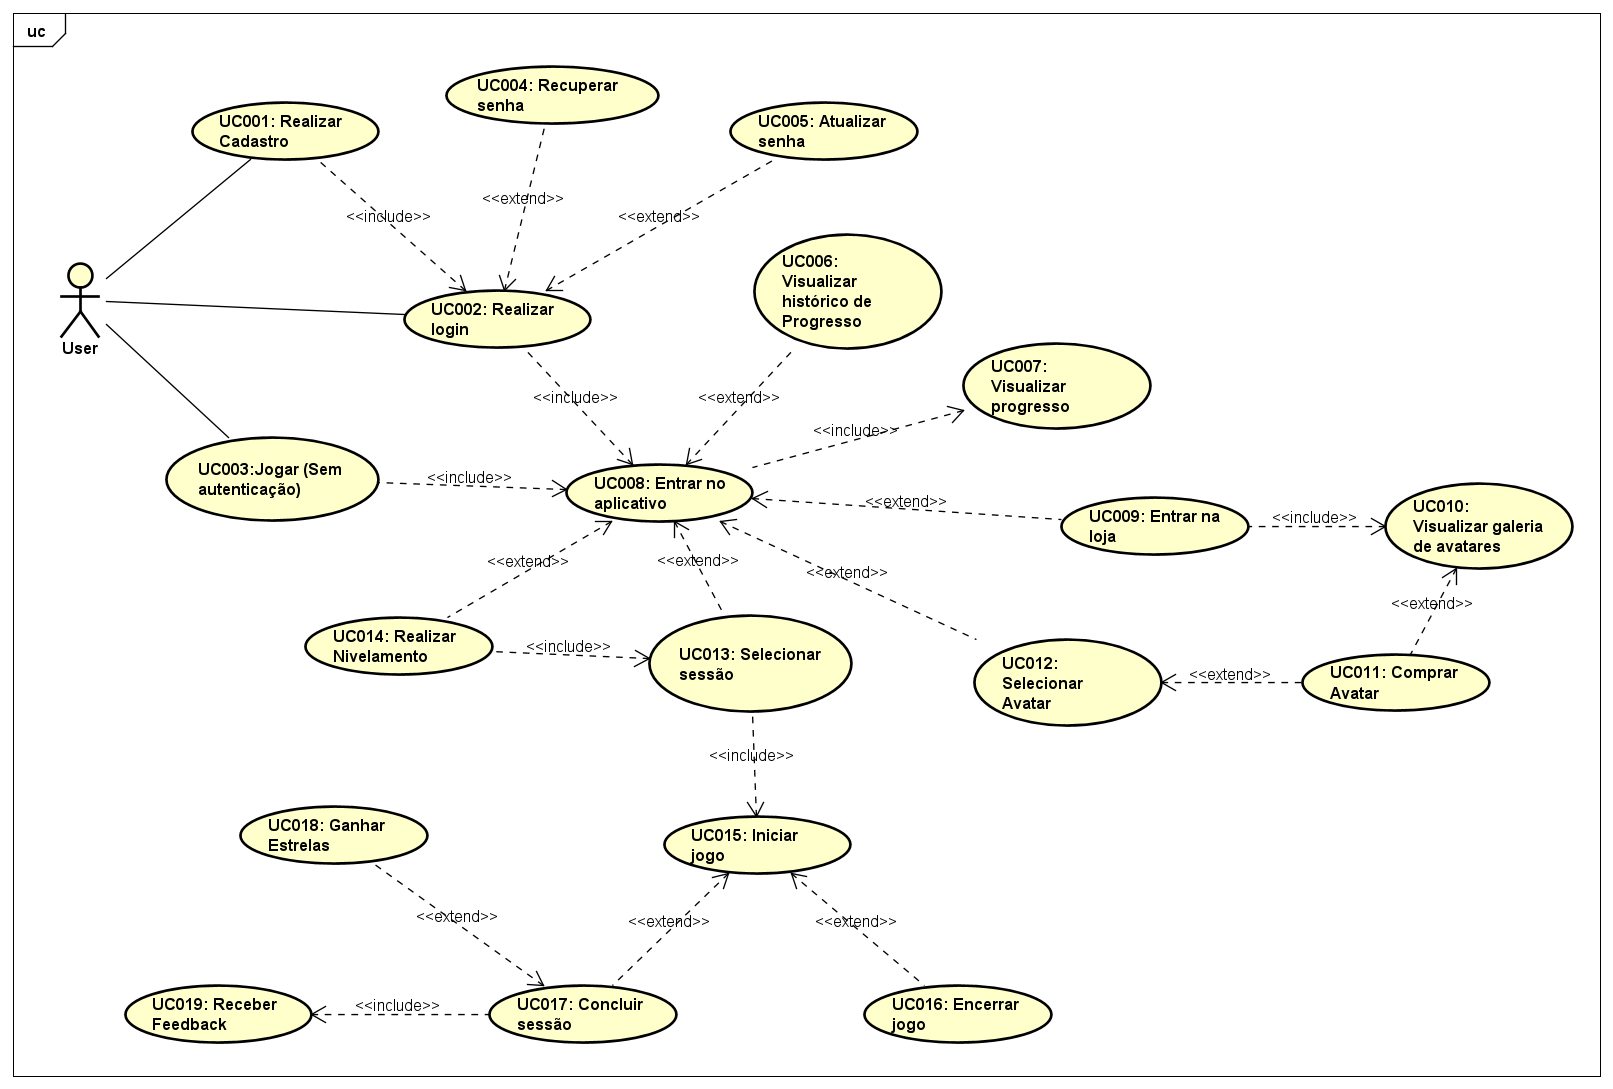
\includegraphics[width=\linewidth]{figuras/UseCase_TCC-1.png}
    \captionof{figure}{Diagrama de caso de uso Fonte: Autores}

    \label{fig:nome-da-imagem}
\end{center}
        \item \textbf{Diagrama de Classes}
        \item \textbf{Diagrama de Atividades}
    \end{itemize}
\end{itemize}

\section{Ferramentas e Tecnologias}

Na presente seção, serão detalhadas as diversas ferramentas e tecnologias empregadas na condução desta pesquisa, desempenhando um papel essencial na coleta, análise e desenvolvimento da pesquisa. A escolha criteriosa desses recursos é fundamental para a robustez e eficácia do estudo, proporcionando uma base sólida para a consecução dos objetivos propostos.

\begin{itemize}

    \item \textbf{React Native} 
    \begin{center}
    
\includegraphics[width=0.5\linewidth]{figuras/React Native.png}
    \captionof{figure}{Logo do framework React Native}
    \label{fig:React Native}
    Fonte para o React Native\footnote{\url{https://reactnative.dev/}}
\end{center}

O React Native é um framework de desenvolvimento de aplicativos móveis que permite a criação de aplicativos nativos para iOS e Android usando JavaScript e React.

A interface foi construída com componentes React Native, possibilitando alta reusabilidade e facilidade de manutenção. O gerenciamento de estado global foi feito via Context API e hooks. Para estilização, usou-se Styled Components com tematização adaptável. A lógica do jogo e regras foram implementadas em JavaScript puro. Atenção especial foi dada à acessibilidade e aspectos cognitivos do público-alvo. O código está organizado seguindo as melhores práticas de React, com componentes pequenos e funções puras. Para qualidade, adotou-se tipagem, testes unitários e integração contínua.No geral, a stack adotada demonstrou alta produtividade e capacidade de entregar uma experiência cross-platform de alto nível e alinhada às necessidades do projeto.

Sobre as versões utilizadas o projeto demonstra o desenvolvimento de um app React Native com recursos avançados de UI, navegação, mídia e animações. O uso do Expo simplifica o setup e configuração do ambiente de desenvolvimento. As versões recentes das principais dependências indicam que o projeto segue as melhores práticas para React Native. No geral, ilustrando um app mobile robusto e bem estruturado utilizando a biblioteca React Native e o ecossistema de ferramentas adjacentes. Utilizando a versão do react 18.2.0 e a versão do react native 0.71.3. 

\begin{itemize}

    \item \textbf{Docusaurus} 
    \begin{center}
    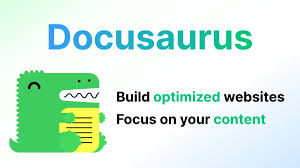
\includegraphics[width=0.5\linewidth]{figuras/Docusaurus.jpg}
    \captionof{figure}{Logo do framework Docusaurus}
    \label{fig:Docusaurus}
    Fonte para o Docusaurus\footnote{\url{https://docusaurus.io/}}
\end{center}

Docusaurus é considerado um framework, especificamente projetado para criar sites de documentação técnica e blogs. Ele facilita a construção de sites estáticos otimizados, integrando Markdown com componentes React, e oferece funcionalidades como tradução, versionamento e busca de conteúdo, permitindo uma personalização avançada e uma experiência de usuário eficiente.O Docusaurus, construído com React, permite personalização avançada e extensão dos layouts do projeto, possibilitando a criação de componentes interativos embutidos nos documentos. Utilizando MDX, integra Markdown com JSX, facilitando a criação de experiências de documentação interativas e ricas. Com seu sistema de versionamento, mantém a documentação sincronizada com as diferentes versões do projeto, garantindo acesso às informações corretas para cada versão do software. 


Suporta internacionalização nativa, permitindo a criação e manutenção de documentação em vários idiomas. Implementa busca de conteúdo usando Algolia, facilitando a localização de informações pelos usuários. Sua arquitetura modular permite o uso de plugins para funcionalidades específicas, como integração com OpenAPI através do plugin Redocusaurus, ou realce de código com Shiki. Oferece uma experiência de desenvolvimento otimizada com recarregamento a quente, construção incremental rápida e fácil implantação em serviços como GitHub Pages, Netlify e Vercel. Além disso, gera arquivos HTML estáticos para cada caminho, otimizando as páginas para motores de busca e ajudando os usuários a encontrar a documentação mais facilmente. A tematização flexível permite personalizar variáveis de CSS, fornecer folhas de estilo próprias e implementar temas personalizados desde o início.

    
    \item \textbf{Expo}
    \begin{center}
    
\includegraphics[width=0.5\linewidth]{figuras/Expo Framework.jpeg}
    \captionof{figure}{Logo do framework Expo}
    \label{fig:Expo}
    Fonte para o Expo Framework\footnote{\url{https://expo.dev/}}
\end{center}

O Expo é uma plataforma para simplificar o desenvolvimento de aplicativos móveis, especialmente em React Native. Ele oferece facilidade de configuração, desenvolvimento sem necessidade de compilação, bibliotecas prontas para uso e ferramentas como o Expo Client para testar aplicativos de forma rápida. O Expo é uma escolha popular para desenvolvedores que buscam uma abordagem simplificada e eficiente no desenvolvimento móvel.

    \item \textbf{Firebase}
    \begin{center}
    
\includegraphics[width=0.5\linewidth]{figuras/Firebase.png}
    \captionof{figure}{Logo do Firebase}
    \label{fig:Firebase}
    Fonte para o Firebase\footnote{\url{https://firebase.google.com/}}
\end{center}

O Firebase é uma plataforma de desenvolvimento de aplicativos da Google que oferece uma variedade de serviços prontos para uso, como autenticação, banco de dados em tempo real, armazenamento de arquivos, hospedagem e mensagens em nuvem. Ele simplifica o desenvolvimento, permitindo que os desenvolvedores integrem funcionalidades essenciais aos seus aplicativos sem a necessidade de configurar servidores complexos. O Firebase é conhecido por sua facilidade de uso e escalabilidade, sendo uma escolha popular para o desenvolvimento rápido de aplicativos web e móveis.

O Firebase fornece uma excelente plataforma de backend como serviço (BaaS) para o projeto. Ele permite o armazenamento de dados na nuvem em tempo real, autenticação de usuários, notificações push e análise de dados, entre outros recursos. Isso simplifica muito o desenvolvimento do aplicativo, pois lida com toda a infraestrutura do backend. Além disso, tem integração nativa com dispositivos Android e iOS, o que é ideal para este projeto mobile. Como o foco está na experiência de aprendizado gamificada, permite que a equipe se concentre na construção da melhor interface e jogabilidade sem se preocupar com complexidades de backend. Portanto, é uma excelente escolha como BaaS para este projeto educacional.


    \item \textbf{TypeScript}
    \begin{center}
    
\includegraphics[width=0.5\linewidth]{figuras/TypeScript.png}
    \captionof{figure}{Logo do TypeScript}
    \label{fig:TypeScript}
    Fonte para a documentação do TypeScript\footnote{\url{https://www.typescriptlang.org/docs/handbook/typescript-in-5-minutes.html}}
\end{center}

O TypeScript é uma linguagem de programação amplamente adotada no desenvolvimento de aplicativos web e mobile. Sua popularidade se deve ao fato de ser um superconjunto tipado do JavaScript, agregando segurança e produtividade à linguagem original. Quando combinado ao framework React Native, o TypeScript se mostra uma excelente escolha para projetos mobile.

Uma das principais vantagens de utilizá-lo com React Native é a capacidade de reaproveitar código entre plataformas. Como o TypeScript é compilado para JavaScript, linguagem nativa do React Native, os desenvolvedores conseguem compartilhar a maior parte do código entre iOS e Android. Isso aumenta a eficiência no desenvolvimento de apps multiplataforma.

Além disso, Typescript possui um vasto ecossistema de bibliotecas e frameworks, incluindo aqueles voltados para React Native. Essas ferramentas facilitam a implementação de recursos como animações, gerenciamento de estado e integração com APIs. A comunidade ativa contribui com tutoriais, documentações e fóruns de discussão, provendo amplo suporte ao desenvolvimento.

Ao optar pelo Typescript com React Native, os desenvolvedores garantem uma linguagem versátil e uma plataforma robusta para a criação de apps modernos e de alta qualidade. A união dessas tecnologias permite um fluxo ágil e produtivo, entregando ao usuário final uma experiência enriquecida. Portanto, o Typescript se consolida como uma ótima escolha para projetos mobile com React Native.

O projeto é um exemplo de aplicação das modernas práticas de desenvolvimento de software. Ele segue uma arquitetura modular, que permite uma maior facilidade de manutenção e extensão do código. O projeto é todo escrito em TypeScript, uma linguagem que oferece segurança de tipo e evita erros comuns em JavaScript.
Além disso conta com o apoio de diversas bibliotecas de terceiros, que fornecem funcionalidades adicionais, como gerenciamento de estado com Redux, roteamento com React Navigation, persistência de dados com AsyncStorage, entre outras. Para garantir a qualidade e a confiabilidade do código, o projeto possui uma suíte abrangente de testes, que utiliza ferramentas como Jest, Enzyme e Detox, facilitando o desenvolvimento e manutenção da aplicação em si.

Por que TypeScript?

    O TypeScript é uma variação do JavaScript que traz benefícios como:

    Tipagem Estática: Ajuda a evitar erros comuns, tornando o código mais claro.

    Melhoria na Segurança e Eficiência: O compilador pode detectar e corrigir erros de tipo em tempo de compilação, economizando tempo na depuração.

    Escalabilidade: Torna o código mais modular e reutilizável, melhorando a escalabilidade.

    \item \textbf{Astah UML}
    \begin{center}
    
\includegraphics[width=0.5\linewidth]{figuras/Astah UML.png}
    \captionof{figure}{logo da ferramenta para criação de UMLs AstahUML }
    \label{fig:Astah UML}
    Fonte para o AstahUML\footnote{\url{https://astah.net/products/astah-uml/}}
\end{center}

O Astah UML é uma ferramenta de modelagem UML (Unified Modeling Language) que oferece recursos abrangentes para profissionais de software, analistas de sistemas e outros envolvidos no desenvolvimento de software. Ele suporta todos os principais diagramas da UML, incluindo diagramas de classe, sequência, atividade, estado, e muito mais. Isso permite que os usuários visualizem e documentem diferentes aspectos de um sistema.
    \item \textbf{Figma}
    \begin{center}
    
\includegraphics[width=0.5\linewidth]{figuras/Figma.png}
    \captionof{figure}{logo da ferramenta de Design Figma}
    \label{fig:Figma}
    Fonte para o Figma Fonte\footnote{\url{https://www.figma.com/}}
\end{center}

O Figma é uma plataforma de design colaborativo baseada na web que revoluciona a maneira como equipes de design trabalham. Permitindo colaboração em tempo real, prototipagem interativa e a criação de bibliotecas de componentes reutilizáveis, o Figma oferece uma abordagem flexível e centrada na equipe para o design de interfaces de usuário (UI) e experiência do usuário (UX). Sua facilidade de uso, ampla compatibilidade com formatos de arquivo e integração fluida com outras ferramentas fazem dele uma escolha popular para profissionais de design e desenvolvimento em todo o mundo.

O Figma foi utilizado para diagramar os wireframes das principais telas e fluxos de navegação do aplicativo. Isso permitiu testar rapidamente como o usuário interage com os elementos de gamificação e conteúdos didáticos já neste estágio inicial. O wireflow desenvolvido no Figma serviu como guia para o desenvolvimento visual e codificação do aplicativo, garantindo que o produto final atendesse às necessidades dos usuários. O protótipo interativo criado também facilitou testes com usuários reais ainda nas fases iniciais do projeto e serviu como base para a evolução da aplicação, fornecendo feedback valioso antes de escrever qualquer linha de código a fim de validações. Seguimos o layout fornecido como base para a implementação. 

Os fluxos de navegação também ajudam a comunicar a jornada do usuário para a equipe, pois permitem visualizar o caminho que um usuário irá percorrer ao realizar determinadas ações. A combinação de wireframes e fluxos de navegação no Figma torna a prototipação uma etapa crucial no processo de design, permitindo uma melhor compreensão das interações e proporcionando uma base sólida para o desenvolvimento do produto.
   
\end{itemize}

\section{Prototipação de telas}

A prototipação de telas é uma etapa importante no design de aplicativos e sites, que permite simular a experiência do usuário antes mesmo de construir o produto final. O protótipo consiste em um modelo interativo das telas, contendo os fluxos de navegação e os elementos de interface. Ele pode ter diferentes níveis de fidelidade, desde esboçosSimples até designs mais refinados. 

A grande vantagem da prototipação é permitir testar e validar ideias de forma rápida e barata, identificando problemas na experiência do usuário precocemente, antes de partir para a programação. Ferramentas como Figma, Adobe XD e Proto.io facilitam a criação de protótipos clicáveis que simulam os comportamentos da interface. Com testes iterativos envolvendo usuários reais, o protótipo é aprimorado até chegar em um design pronto para ser desenvolvido. Dessa forma, a prototipação ajuda a economizar tempo e evitar retrabalho no processo de design.

Transcende sua função primordial e se transforma em uma poderosa ferramenta de aprendizado. Imagine seus alunos imersos no processo de design, contribuindo com ideias e feedbacks valiosos. Essa experiência única contribui para o desenvolvimento de habilidades essenciais como pensamento crítico e resolução de problemas, além de aumentar significativamente o engajamento com o aplicativo.

\subsection{Desenvolvimento do protótipo}


\begin{itemize}
    \item \textbf{Participantes e procedimentos da avaliação do protótipo}
    \item \textbf{Validação: testes de usabilidade, observação de uso, feedback dos usuários}
    
\end{itemize}

\section{Repositório}

O que é um Repositório?

Um repositório no GitHub é como um cofre para seu projeto. Ele contém todos os arquivos do seu projeto, além do histórico de todas as alterações feitas ao longo do tempo. É como uma versão online do seu projeto que facilita a colaboração e o controle de versões.

Estrutura do Repositório

Branches

No contexto do GitHub, usamos "branches" para criar diferentes versões do projeto. Cada branch é uma ramificação independente do código-fonte, possibilitando que você isole e desenvolva novas funcionalidades, refatore o código ou faça correções e testes em paralelo, sem interferir no código existente na branch principal, que geralmente é nomeada como \textit{main} \cite{al}. Neste projeto, utilizamos apenas a branche \textit{main}.


Refatoração e Aprimoramento

Uma análise crítica da estrutura existente levou a mudanças significativas. A reestruturação do código, adotando melhores práticas e aprimorando a arquitetura. Bem como a criação de uma nova branche nomeada de develop ...................

E o projeto ficou organizado da seguinte maneira: 

Branche main

............

Branche develop

..............

Versionamento do Código

Versão 0.0.1 -  Criação do projeto.

Versão 0.1.0 - Organizamos as pastas de forma mais lógica. Cada tipo de funcionalidade agora tem seu próprio espaço. Para facilitar a compreensão e manutenção do código.

Versão 0.2.0 - Componentização. Dividimos os componentes em partes menores, cada uma realizando uma tarefa específica. Isso ajuda na organização e na compreensão do código.

Versão 0.3.0 - Separamos os arquivos de estilo, proporcionando uma consistência visual melhor.

Versão 0.4.0 - Movemos o gerenciamento de estado para "stores", proporcionando uma prática recomendada para projetos React Native.

Versão 1.0.0-alpha - Decidimos mudar a tecnologia utilizada de JavaScript para TypeScript.


Onde usar?  ->  Essas mudanças visavam criar uma base de código mais organizada, fácil de entender e pronta para receber atualizações e melhorias no futuro. Este projeto, agora utilizando TypeScript e seguindo melhores práticas, está mais preparado para crescer de maneira sustentável e com qualidade.










\subsection{Guia de navegação da Landing Page - Seções Principais}



Landing Page é um página web focada em apresentar a missão e os benefícios da aplicação, incentivando os visitantes a se envolverem. Ela busca converter visitantes em usuários ativos através de ações como cadastro ou download do material apresentado.

Para melhor entendimento e resumo do projeto foi criado uma Landing Page com o intuito de concentrar os principais pontos da idealização e facilitar a interação com os alunos e professores ela pode ser acessada atráves do site mencionado abaixo na figura 9. 


\subsection{1. Documentação}
\begin{itemize}
    \item Localizada na barra lateral sob ``Sobre o projeto''
    \item Contém documentação principal do projeto
    \item Acessível pela barra de navegação superior ou barra lateral
\end{itemize}

\subsection{2. Tecnologias Utilizadas}
Detalhamento das principais tecnologias:
\begin{itemize}
    \item \textbf{Docusaurus}: Plataforma de documentação
    \item \textbf{Next.js}: Framework web
    \item \textbf{Firebase}: Serviços de backend
    \item \textbf{React Native}: Desenvolvimento mobile
\end{itemize}

\subsection{3. Recursos do Projeto}
Acessível via navegação lateral:
\begin{itemize}
    \item Objetivos do projeto
    \item Diagramas de classe
    \item Requisitos funcionais/não-funcionais
    \item Protótipos (Figma)
\end{itemize}

\subsection{4. Como Contribuir}
Localizado em ``Como contribuir com o projeto?'':
\begin{itemize}
    \item Formulários de feedback
    \item Instruções para testes
    \item Como reportar problemas
\end{itemize}

\section{Elementos de Navegação}

\subsection{Barra Superior}
\begin{itemize}
    \item Link para documentação
    \item Link para repositório GitHub
\end{itemize}

\subsection{Barra Lateral}
\begin{itemize}
    \item Organização hierárquica com seções:
    \begin{itemize}
        \item Documentação
        \item Informações técnicas
        \item Diretrizes de contribuição
    \end{itemize}
\end{itemize}

\subsection{Elementos Interativos}
\begin{itemize}
    \item Visualização de protótipos
    \item Formulários de feedback
    \item Links para download
\end{itemize}

\subsection{Rodapé}
\begin{itemize}
    \item Recursos adicionais
    \item Links da comunidade
    \item Informações de copyright
\end{itemize}

\section{Elementos de Navegação}

\subsection{Barra Superior}
\begin{itemize}
    \item Link para documentação
    \item Link para repositório GitHub
\end{itemize}

\subsection{Barra Lateral}
\begin{itemize}
    \item Organização hierárquica com seções:
    \begin{itemize}
        \item Documentação
        \item Informações técnicas
        \item Diretrizes de contribuição
    \end{itemize}
\end{itemize}

\subsection{Elementos Interativos}
\begin{itemize}
    \item Visualização de protótipos
    \item Formulários de feedback
    \item Links para download
\end{itemize}

\subsection{Rodapé}
\begin{itemize}
    \item Recursos adicionais
    \item Links da comunidade
    \item Informações de copyright
\end{itemize}

    \item \textbf{Landing Page - Math.Pow}
    \begin{center}
    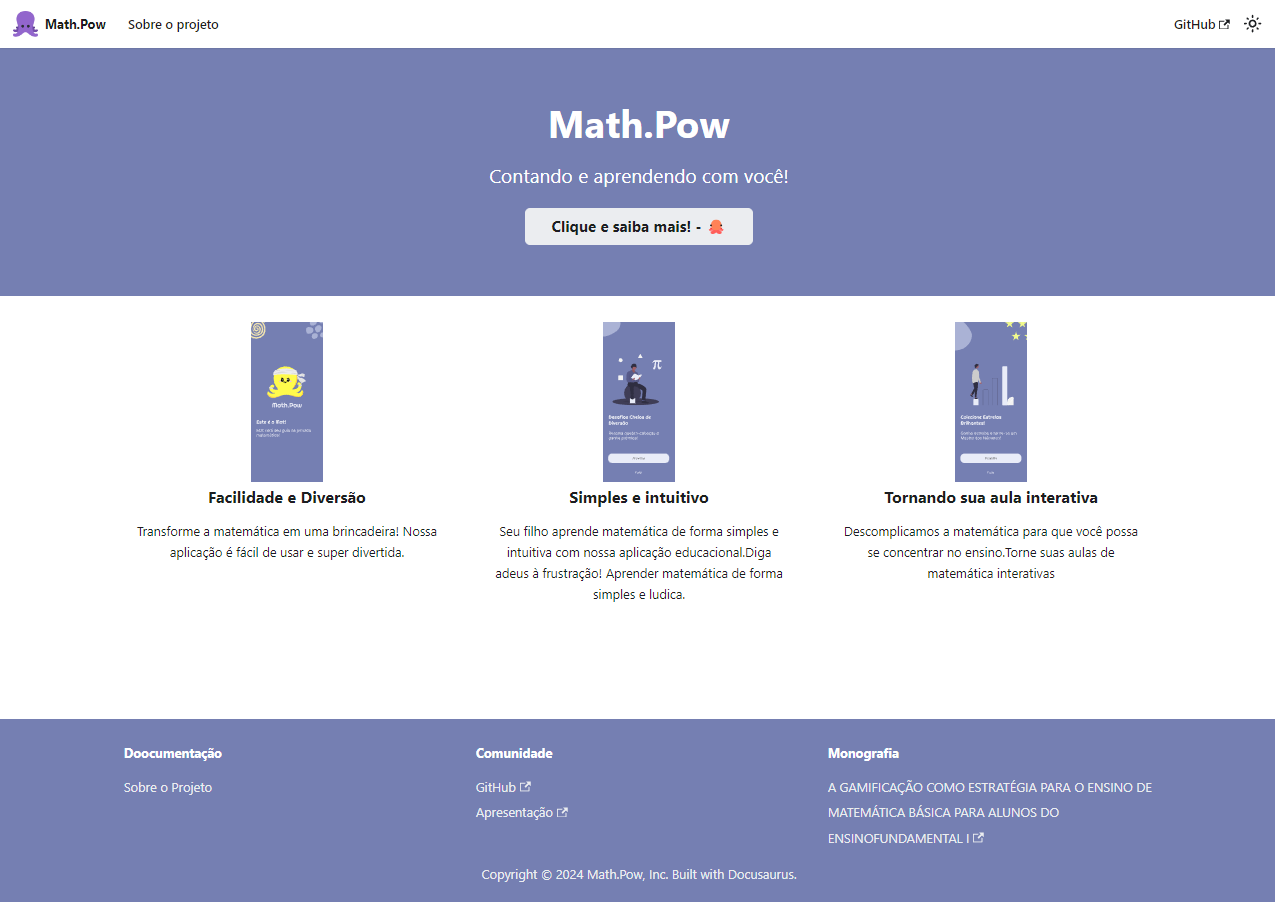
\includegraphics[width=0.8\linewidth]{figuras/Math.Pow App/mathPow.png}
    \captionof{figure}{Imagem do site do projeto}
    \label{fig:Figma}
    Fonte para a página do projeto Fonte\footnote{\url{https://mathpow.vercel.app/
\end{center}


 
